% ============================================================
%  SCHOLA DOMESTICA — Level 1, Week 2, Lesson 8
%  Topic: Number 10 — A Complete Group
%  8–10 problems | No speed drill | Picture-heavy
%  Compile with XeLaTeX
% ============================================================
\documentclass[12pt,letterpaper]{article}
\usepackage{../sd_style}

\renewcommand{\lessonnum}{8}
\renewcommand{\lessonweek}{2}

\begin{document}

\lessonheader{2}{8}{The Number 10}

\begin{instructbox}
\noindent\textbf{\color{sd-blue}Instruction} \textit{(read aloud):}\\[4pt]
Today we meet \textbf{10} — a very special number!
Ten is a whole group: all ten fingers, all ten toes.
Ten is written with a \textbf{1} and a \textbf{0} together.
The 1 means one group of ten, and the 0 means no extra ones.
\end{instructbox}

\vspace{8pt}
\noindent\textbf{\color{sd-blue}Trace and write:}
\tracerowone{10}

\vspace{6pt}
% Ten-frame visual
\noindent\textbf{\color{sd-blue}Ten-frame:} \textit{Count the filled squares — that is ten!}
\vspace{6pt}

\begin{center}
\begin{tikzpicture}
  \foreach \x in {0,...,4}{
    \draw[sd-blue, thick] (\x*1.1, 0) rectangle (\x*1.1+0.9, 0.9);
    \draw[sd-blue, thick] (\x*1.1, 1.1) rectangle (\x*1.1+0.9, 2.0);
    \fill[sd-gold] (\x*1.1+0.45, 0.45) circle (0.32);
    \fill[sd-gold] (\x*1.1+0.45, 1.55) circle (0.32);
  }
\end{tikzpicture}
\end{center}

\goldrule
\noindent\textbf{\color{sd-blue}Practice}
\vspace{6pt}

\prob Count the dots.\\[6pt]
\hspace{1cm}\onedot\onedot\onedot\onedot\onedot\onedot\onedot\onedot\onedot\onedot\quad\ansblank

\vspace{10pt}
\prob How many fingers do you have in all?\\[4pt]
\hspace{1cm}\IfFileExists{hands_10.jpg}{\includegraphics[height=2cm]{hands_10.jpg}}{%
  \textit{[Hold up both hands]}}
\quad\ansblank

\vspace{10pt}
\prob How many?\\[4pt]
\hspace{1cm}\IfFileExists{stars_10.jpg}{
\includegraphics[height=1.4cm]{stars_10.jpg}}{%
  \onestar\onestar\onestar\onestar\onestar\onestar\onestar\onestar\onestar\onestar}
\quad\ansblank

\vspace{10pt}
\prob Circle the group of \textbf{10}.\\[6pt]
\begin{center}
\begin{tabular}{ccc}
\textbf{A}\quad%
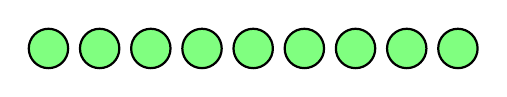
\begin{tikzpicture}[baseline=0]
  \foreach \x in {0,...,8}\draw[fill=green!50,thick](\x*0.65,0)circle(0.25);
\end{tikzpicture}
&\quad\quad&
\textbf{B}\quad%
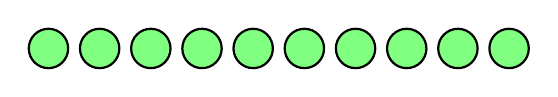
\begin{tikzpicture}[baseline=0]
  \foreach \x in {0,...,9}\draw[fill=green!50,thick](\x*0.65,0)circle(0.25);
\end{tikzpicture}
\end{tabular}
\end{center}

\vspace{10pt}
\prob Write the number 10 four times, your neatest writing:\\[6pt]
\noindent\fbox{\rule{0pt}{1.6cm}\hspace{11cm}}

\vspace{10pt}
\prob \textit{(Teacher reads)} There were 7 goldfish in the pond.
Three more swam in. How many goldfish now? \quad\ansblank

\vspace{10pt}
\prob Write the numbers in order from 1 to 10:\\[6pt]
\hspace{1cm}\ansblank\quad\ansblank\quad\ansblank\quad\ansblank\quad\ansblank\quad%
\ansblank\quad\ansblank\quad\ansblank\quad\ansblank\quad\ansblank

\vspace{10pt}
\prob What number comes just before 10? \quad\ansblank

\goldrule

\begin{checkbox}
\noindent\textbf{\color{sd-green}Knowledge Check}\\[4pt]
\setcounter{probnum}{0}
\prob Count to 10 aloud for your teacher. \quad $\square$~Done\\[8pt]
\prob Write the number ten: \quad\ansblank \quad
  How many digits does it use? \quad\ansblank
\end{checkbox}

\vfill
\noindent{\color{sd-blue}$\bigstar$ \textbf{Enrichment — Roman Numerals:}}\\
The Romans wrote ten as \textbf{X} — two V's crossed together (V = 5, and 5+5 = 10).\\[4pt]
\begin{tabular}{cccccccccc}
\textbf{I}&\textbf{II}&\textbf{III}&\textbf{IV}&\textbf{V}&
\textbf{VI}&\textbf{VII}&\textbf{VIII}&\textbf{IX}&\textbf{X}\\
1&2&3&4&5&6&7&8&9&10
\end{tabular}\\[4pt]
Can you write I through X from memory?\\[4pt]
\noindent\fbox{\rule{0pt}{1.4cm}\hspace{11cm}}

\vspace{4pt}\hrule\vspace{3pt}
{\footnotesize\color{gray}\textit{Teacher note: Ten is the cornerstone of our number system.
  Spend extra time if needed — strong understanding of ten as a unit is essential
  for all future place value work. A physical ten-frame with counters is ideal.}}

\end{document}
